% Tipo di documento. L'uso di twoside implica che i capitoli inizino sempre con la prima pagina a sinistra, eventualmente lasciando una pagina vuota nel capitolo precedente. Se questa cosa è fastidiosa, è possibile rimuoverlo. 
\documentclass[a4paper,openright]{report}

% Dimensione dei margini
\usepackage[a4paper,top=3cm,bottom=3cm,left=3cm,right=3cm]{geometry} 
% Dimensione del font
\usepackage[fontsize=12pt]{scrextend}
% Lingua del testo
\usepackage[italian,english]{babel}
% Lingua per la bibliografia
% \usepackage[fixlanguage]{babelbib}
% Codifica del testo
\usepackage[utf8]{inputenc} 
% Font mono (quello di default non supporta il grassetto)
\usepackage{courier}
% Encoding del testo
\usepackage[T1]{fontenc}
% Lorem Ipsum
\usepackage{lipsum}
% Bibliografia
\usepackage[
backend=biber,
bibstyle=other/custom-numeric,
citestyle=numeric,
sorting=none,
]{biblatex}
% Sorgente della bibliografia
\addbibresource{chapters/Bibliography.bib}
% Per ruotare le immagini
\usepackage{rotating}
% Per cambiare i capitoli
\usepackage{titlesec}
\titleformat{\chapter}[hang]
  {\normalfont\bfseries\huge}{\thechapter}{1em}{\huge}
% Per mostrare nell'indice anche le subsubsection
\setcounter{tocdepth}{3}
% Per modificare l'header delle pagine 
\usepackage{fancyhdr}
% Librerie matematiche
\usepackage{amssymb}
\usepackage{amsmath}
\usepackage{mathtools}
\usepackage{amsthm}         
% Uso delle immagini
\usepackage{graphicx}
% Uso dei colori
\usepackage[dvipsnames,svgnames,x11names]{xcolor}
% Uso dei listing per il codice
\usepackage{listings}          
% Per inserire gli hyperlinks tra i vari elementi del testo 
% \usepackage[hang, flushmargin]{footmisc}
% Diversi tipi di sottolineature
\usepackage[normalem]{ulem}
% Fix relative indenting
\usepackage{lstautogobble}
% Code coloring
\usepackage{color}
% Nice font
\usepackage{zi4}
% Loads the Latin Modern font
\usepackage{lmodern}
% For text alignment
\usepackage{ragged2e}
% Customizes the appearance of figure and table captions
\usepackage{caption}
% Code highlighting
\usepackage[newfloat,outputdir=out]{minted}
% Better frame for minted
\usepackage{tcolorbox}
\tcbuselibrary{minted,skins,breakable,xparse}
\tcbuselibrary{listingsutf8} % Allows minted in tcolorbox
% Additional options to control the placement of figures and tables
\usepackage{float}
% No paragraph indentation instead vspaces
\usepackage[skip=5pt]{parskip}
% Allows customization of line spacing
\usepackage{setspace}
% Enables switching or substituting hyphenation patterns in your document
\usepackage{hyphsubst}
% Improves the overall typography of the document by subtly adjusting spacing and font shapes
\usepackage{microtype}
% Allows the creation of hyperlinks in the document
\usepackage{hyperref}
% Adds back-references from footnotes to the point in the text where the footnote was used
\usepackage{footnotebackref}
% Tools for formatting and managing quotes in your document
% To be used after minted
\usepackage{csquotes}
% Adding sub-captions to figures and tables
\usepackage{subcaption}
% Drawing electrical and electronic circuit diagrams
\usepackage{circuitikz}
% Permits to patch macros
\usepackage{xpatch}

\usepackage{multirow}
\usepackage{booktabs}
\usepackage{siunitx} % For proper unit formatting
\usepackage{cleveref} % For proper unit formatting


% Comments ( substitute command name and name )
\newcommand{\cuno}[1]{\textcolor{red}{[\bfseries Persona 1: #1]}}
\newcommand{\cdue}[1]{\textcolor{red}{[\bfseries Persona 2: #1]}}

% Don't include in \leftmark "Chapter"
\renewcommand{\chaptermark}[1]{%
  \markboth{\thechapter. #1}{}%
}
% Modifica lo stile dell'header
\pagestyle{fancy}
\fancyhf{}
% These work if the document is in twoside mode
% \fancyhead[CE,CO]{\rightmark}
% \fancyhead[LE,RO]{\textbf{\thepage}}

% Make the header
% on the left side, show the chapter title if no section is present, otherwise the section title
% on the right side, show the page number
\fancyhead[L]{
  \ifnum\value{section}=0 % Check if no section exists
    \leftmark            % Use Chapter title
  \else
    \rightmark           % Use Section title
  \fi
}
\fancyhead[R]{\textbf{\thepage}}
\fancyfoot{}
\setlength{\headheight}{17pt}

% Rimuove il numero di pagina all'inizio dei capitoli
\fancypagestyle{plain}{
  \fancyfoot{}
  \fancyhead{}
  \renewcommand{\headrulewidth}{0pt}
}

% Custom colors
\definecolor{DarkGreen}{RGB}{20,80,40}
\definecolor{Unipi}{RGB}{00,85,143} 
\definecolor{term_bg_color}{RGB}{240,241,240} 

% Modifica dello stile dei riferimenti
\hypersetup{
    colorlinks,
    linkcolor=Unipi,
    citecolor=Unipi,
    urlcolor=Unipi
}

% Interlinea
\setstretch{1.1}

% Supercite tipo wikipedia
\DeclareCiteCommand{\supercite}[\mkbibsuperscript]
  {\iffieldundef{prenote}
     {}
     {\BibliographyWarning{Ignoring prenote argument}}%
   \iffieldundef{postnote}
     {}
     {\BibliographyWarning{Ignoring postnote argument}}}
  {\usebibmacro{citeindex}%
   \bibopenbracket\usebibmacro{cite}\bibclosebracket}
  {\supercitedelim}
  {}


% Aggiunti definizioni, teoremi, linea e listing
\newtheorem{definition}{Definizione}[section]
\newtheorem{theorem}{Teorema}[section]
\providecommand*\definitionautorefname{Definizione}
\providecommand*\theoremautorefname{Teorema}
\providecommand*{\listingautorefname}{Listing}
\providecommand*\lstnumberautorefname{Linea}

\newcommand{\cboh}[1]{{\textcolor{blue}[\textcolor{magenta}{\bf{!!: }}{ \textcolor{blue}{#1]}}}}

% LaTeX stops trying to balance the text across pages, allowing pages to have uneven bottom margins
\raggedbottom

%----------------------------------------------------

\begin{document}

\setlength{\fboxsep}{0pt}
\selectlanguage{english}

% \hyphenpenalty=10000
% \exhyphenpenalty=10000

% \loadspellchecklist[it][wordlist.txt]
% \setupspellchecking[state=start]


% Define a custom style for your tcolorbox
\tcbset{
    listing engine=minted,
    minted options={
            fontsize=\small,
            linenos,
            numbersep=4mm,
            breaklines,
            baselinestretch=0.9
        },
    colback=term_bg_color,
    colframe=Unipi,
    fonttitle=\bfseries,
    listing only,
    left=1.5mm,
    arc=0.5mm,
    enhanced,
    breakable,
    before skip=\baselineskip,
    grow to left by=2mm,grow to right by=2mm,
    enlarge bottom by=-8pt
}

% Define command to include a minted file
\newtcbinputlisting{\mintedCode}[3][]{%
    listing file={#3},
    minted language={#2}
}

% Space between caption and figure, listing
\setlength{\abovecaptionskip}{8pt}
\setlength{\belowcaptionskip}{6pt}
\captionsetup[figure]{belowskip=-12pt}

% Define a new environment for code listings
\newenvironment{code}
{\captionsetup{type=listing}}
{\par\noindent\ignorespacesafterend}

\SetupFloatingEnvironment{listing}{name=Listing, listname=List of Listings}

\usemintedstyle{sas}
% \usemintedstyle{unipi}
% \usemintedstyle{xcode}
% \usemintedstyle[output]{rrt}


\begin{titlepage}
\begin{figure}[!htb]
    \centering
    
\includegraphics[keepaspectratio=true,scale=0.5]{images/Frontespizio/cherubinFrontespizio.eps}
\end{figure}

\begin{center}
    \LARGE{UNIVERSITY OF PISA}
    \vspace{5mm}
    \\ \large{MSc in Computer Engineering}
    \vspace{5mm}
    \\ \LARGE{Project for Performance Evaluation of Computer Systems and Networks}
\end{center}

\vspace{15mm}
\begin{center}
    {\LARGE{\bf Multi-core scheduling}}
    
    % Se il titolo è abbastanza corto da stare su una riga, si può usare
    
    % {\LARGE{\bf Un fantastico titolo per la mia tesi!}}
\end{center}
\vspace{30mm}

\begin{minipage}[t]{0.47\textwidth}
	{\large{Professors:}{\normalsize\vspace{3mm}\bf\\ \large{Prof. Giovanni Stea}}{\normalsize\vspace{3mm}
               \bf\\ \large{Ing. Giovanni Nardini }}}

\end{minipage}
\hfill
\begin{minipage}[t]{0.51\textwidth}\raggedleft
	{\large{Students:}
            {\normalsize\vspace{3mm} \bf\\ \large{Taulant Arapi (645308)}}
            {\normalsize\vspace{3mm} \bf\\ \large{Francesco Barcherini (645413)}}
            {\normalsize\vspace{3mm} \bf\\ \large{Antonio Ciociola (645324)}}
        }
            
\end{minipage}

\vspace{30mm}
\hrulefill
\\\centering{\large{ACADEMIC YEAR 2024/2025}}

\end{titlepage}

% \begin{titlepage}
% \begin{figure}[!htb]

% \begin{center}
% {
%     
\includegraphics[keepaspectratio=true,scale=0.5]{images/Frontespizio/cherubinFrontespizio.eps}
% }
% \end{center}

% \end{figure}

% \begin{center}
%     \LARGE{UNIVERSITÀ DI PISA}
% \end{center}

% \vspace{15mm}
% \begin{center}
%     {\LARGE{\bf
%     TITOLO  
%     \\ \vspace{3mm}
%     TITOLO RIGA 2
%     }}
% \end{center}

% \vspace{50mm}


% \begin{minipage}[t]{0.47\textwidth}
% 	{
%         \large{Authors:}
%         {\normalsize\vspace{3mm}\bf\\ 
%         \large{Taulant Arapi}
%         \normalsize\vspace{3mm}\bf \\
%         \large{Francesco Barcherini}
%         \normalsize\vspace{3mm}\bf \\
%         \large{Antonio Ciociola}
%         }
%     }
% \end{minipage}


% \vfill
% \hrulefill
% \\\centering{\large{ANNO ACCADEMICO 2024/2025}}

% \end{titlepage}
\stepcounter{page}

\tableofcontents


\chapter{Photos}

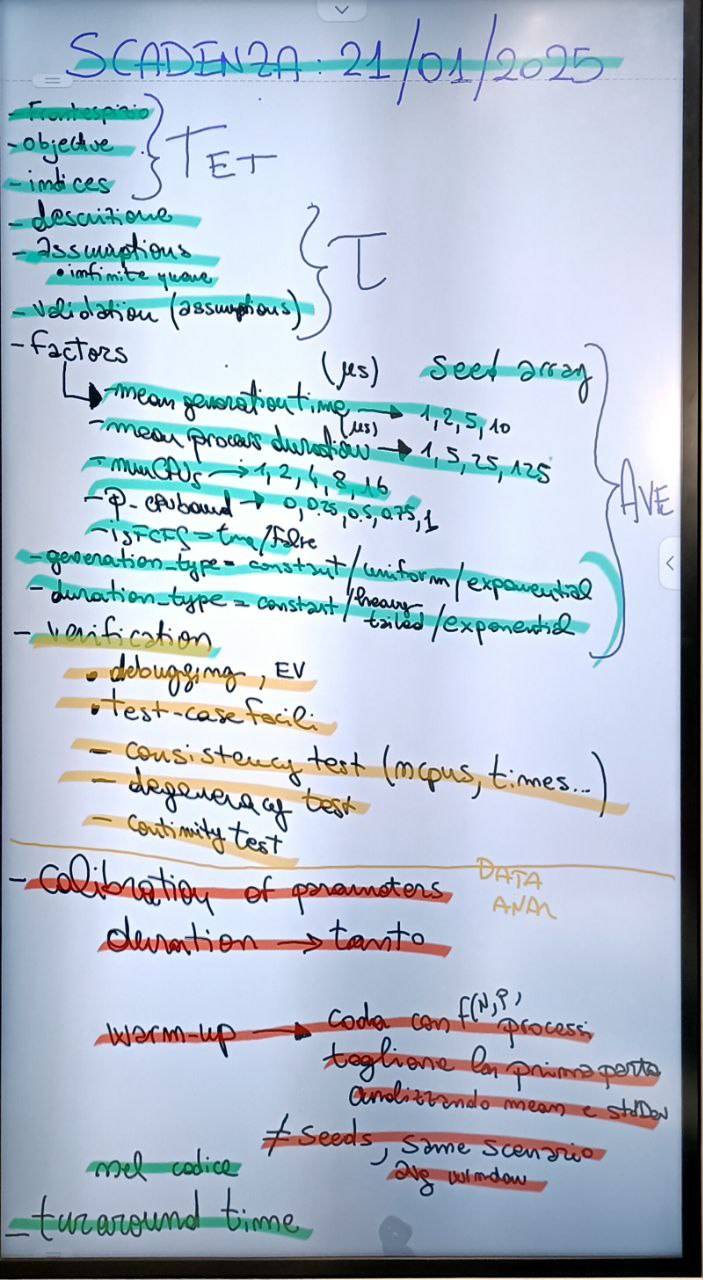
\includegraphics[width=0.6\textwidth]{images/example/pag1.jpeg}
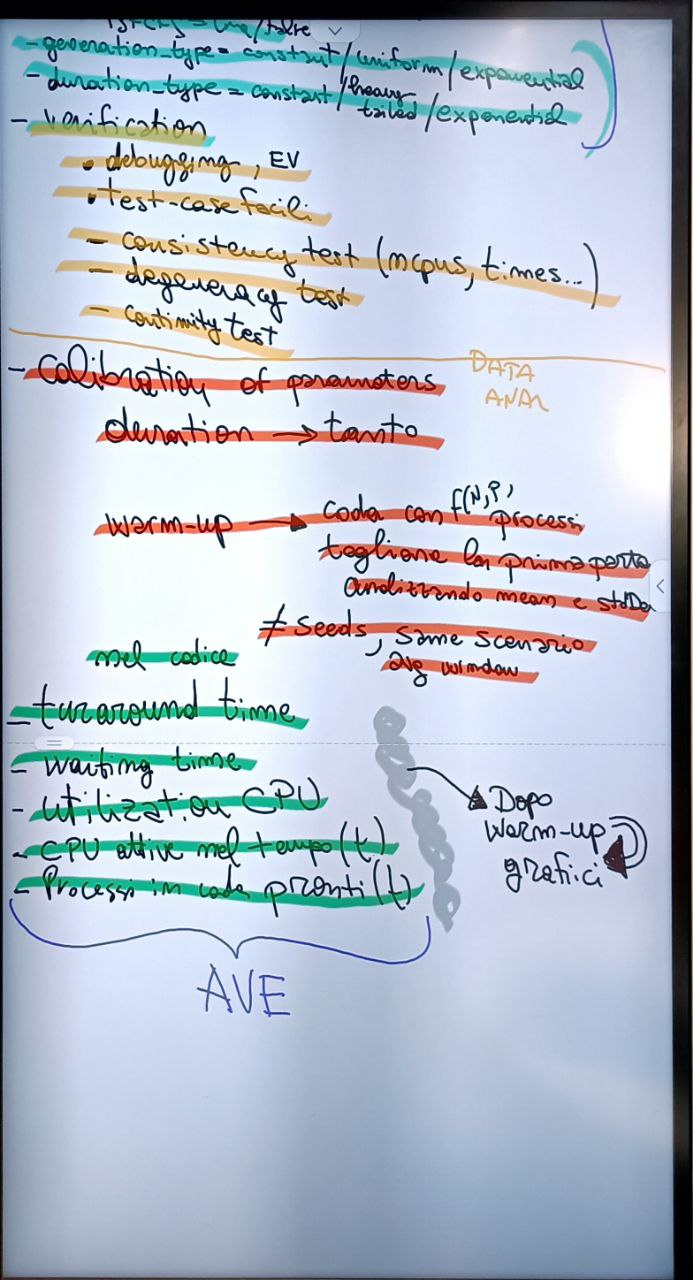
\includegraphics[width=0.6\textwidth]{images/example/pag2.jpeg}
\begin{figure}
    \centering
    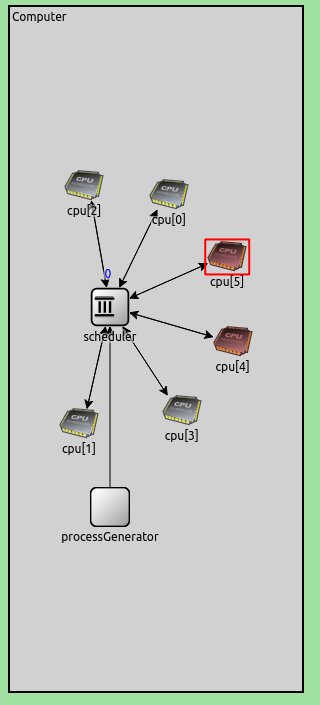
\includegraphics[width=0.7\textwidth]{images/example/sim_schema.png}
    \caption{Caption}
    \label{fig:enter-label}
\end{figure}
\chapter{Introduction}

\section{Description and specification}
It is required to analyze a multi-core computer equipped with \( N \) CPUs, which execute multiple interactive processes. The processes are dynamically generated at intervals of \( T \) seconds. Each process has a total duration \( D \), which is divided into three distinct execution phases:
\begin{enumerate}
    \item initial processing phase;
    \item I/O operation phase;
    \item final processing phase.
\end{enumerate}

The times \( T \) and \( D \) are defined as IID random variables. The processes are categorized into two types and generated as \textit{CPU bound} with probability \( p \) or \textit{I/O bound} with probability \( 1 - p \). The difference is that:
\begin{itemize}
    \item in CPU-bound processes the I/O operation phase constitutes 20\% of the total duration \( D \), and the other two phases both the 40\%;
    \item in I/O-bound processes the I/O operation phase constitutes 80\% of their total duration \( D \), and the other two phases both the 10\%;
\end{itemize}

Processes are assigned to CPUs by the operating system’s scheduler, which selects tasks from a list of “ready” processes. When a CPU becomes idle for entering the I/O operation phase or ending the final processing phase of a process, the scheduler immediately assigns it to a new ready process, if present. Once a process completes its I/O operation phase, it is marked as ready again and is returned to the scheduling queue. A process exits the system once it has successfully completed all three phases of execution.

The scheduler can be implemented to follow two distinct policies:
\begin{itemize}
    \item First Come First Served (FCFS): processes are scheduled in the order of their arrival after the generation or after the end of the I/O phase;
    \item Shortest Job First (SJF): scheduling is determined based on the shortest remaining time until either the process’s I/O phase or its completion.
\end{itemize}

\section{Objectives}

The aim of this project is to assess and analyze the execution of a multi-core scheduling system under varying operational scenarios. The objective is to determine the optimal characteristics of the systems to make it work without the need to discard processes. Furthermore, the analysis aims to assess the conditions under which the best system behavior is achieved in terms of resource use efficiency and time performance evaluation. In particular, the different configurations taken into consideration are the scheduling policies, the number of CPUs in the system, the type of the processes (CPU bound or I/O bound), the generation intervals and the duration of processes.

The overarching goal is to generate insights into optimal scheduling strategies and resource allocation practices for multi-core environments, enhancing system throughput and minimizing delays.


\section{Indices}

To evaluate the system’s performance comprehensively, the following indices will be analyzed in detail:
\begin{itemize}
    \item turnaround time $R$: defined as the total time elapsed from the arrival of a process in the system to its completion. This metric provides a measure of the computer’s overall responsiveness and of the time required for different types of processes to be executed;
    \item waiting time $W$: the cumulative time \cboh{COME LO CALCOLIAMO?} a process spends in the ready queue before being assigned to a CPU for execution. This metric represents the impact on the turnaround time of the queuing policy and of the workload of the system;
    \item CPU utilization of the $n_{th}$ CPU $\rho_n$: the fraction of time that each CPU is actively engaged in executing processes instead of being idle. This metric reflects the efficiency of resource usage within the system;
    \item active CPUs over time $N_A$: a dynamic measure of the number of CPUs actively processing tasks at any given moment. This index helps assess load distribution and system evolution;
    \item queue length over time $N_q$: tracks the size of the ready queue throughout the simulation, highlighting bottlenecks and variations in process scheduling.
\end{itemize}

These indices will be statistically analyzed to identify trends, anomalies, edge cases and key factors influencing system performance. By examining these metrics under diverse configurations of \( N \), \( p \) and scheduler policies, the project aims to provide actionable recommendations for improving the efficiency and adaptability of multi-core scheduling systems.

\section{Assumptions?}
To perform the analysis, the following assumptions are made:
\begin{itemize}
    \item There is sufficient memory to store the list of processes ready for execution, so the ready queue will be considered as infinite.
    \item The scheduler itself has a negligible load on the CPUs; there is no delay between the executions of the modeled processes. \cboh{assumiamo che sia zero? if not, quanto facciamo?}
    \item With the shortest job first (SJF) scheduling, an accurate estimate of the execution times is known a priori. If the scheduler is FCFS, this data is not used.
\end{itemize}
\chapter{Implementation}
We implemented the Computer system in OMNeT++.\\
Our implementation consists of the following modules, also shown in \autoref{fig:omnetpp_implementation}:
\begin{itemize}
    \item \texttt{ProcessGenerator}: this module generates processes following the specified time distribution and sends them to the scheduler. The duration of each processing phase is also defined here.
    \item \texttt{scheduler}: this module handles the scheduling logic and keeps track of processes in their I-O phase.\\
    It contains an infinite-capacity queue. Depending on the \texttt{isFCFS} parameter, the queue is either a FIFO queue, when the parameter is set to true, or a priority queue whose elements are ordered by increasing duration.
    \item \texttt{cpu}: each of the $N$ CPUs, when it is free, receives a process from the scheduler and simulates its execution. When it finishes the execution phase (i.e. the I-O phase is reached or the process terminates), a message is sent to the scheduler, indicating that the CPU is now free.
\end{itemize}

\begin{figure}[H]
    \captionsetup{type=figure}
    \centering
    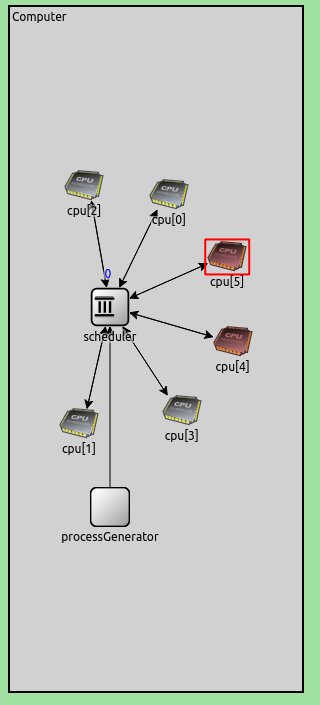
\includegraphics[width=0.4\textwidth]{images/example/sim_schema.png}
    \captionof{figure}{View of the system implementation in OMNeT++}
    \label{fig:omnetpp_implementation}
\end{figure}


\section{Calibration of the factors}

\begin{itemize}
    \item \texttt{meanGenerationTime}: 
    \item \texttt{meanProcessDuration}: 
    \item \texttt{pCpuBound}: 
    \item \texttt{numCpus}: 
    \item \texttt{isFCFS}: 
    \item \texttt{generationType}: 
    \item \texttt{durationType}: 
\end{itemize}

\chapter{Verification}
\chapter{Analysis}

\section{Calibration of the parameters}

Having a lot of parameters to calibrate, we decided to limit the number of possible values for each parameter. This choice was made to reduce the number of simulations to be performed and to have a more manageable number of results to analyze. The parameters that we decided to calibrate are the following:

\begin{itemize}
    \item \texttt{meanGenerationTime}: \{20ms, 50ms\} \\
          The mean for the generation times of the processes was chosen by considering a system under heavy and medium load.
    \item \texttt{meanProcessDuration}: \{40ms, 100ms, 200ms\} \\
          The mean for the duration of the processes was chosen after the estimations on the system stability. These values permit to have some combination of parameters that lead to a stable system and others that lead to an unstable system.
    \item \texttt{pCpuBound}: \{0.25, 0.75\} \\
          The probability of a process being CPU-bound has two values, one for a system with a high number of I-O bound processes and the other for a system with a high number of CPU-bound processes.
    \item \texttt{numCpus}: \{1, 4, 12\} \\
          The number of CPUs was chosen to simulate single-core, quad-core, and newer systems with 12 cores.
    \item \texttt{isFCFS}: \{true, false\} \\
          The scheduling policy that the scheduler uses can be either First-Come-First-Served or Shortest-Job-First.
    \item \texttt{generationType}: \{"exponential", "uniform"\} \\
          In addition to the exponential distribution, we also considered the uniform distribution for the generation of processes.
    \item \texttt{durationType}: \{"exponential", "uniform"\} \\
          In addition to the exponential distribution, we also considered the uniform distribution for the duration of the processes.
\end{itemize}


\section{Time parameters setup}

\subsection{Warm-up period}

To determine the warm-up period, we observed the development of the mean number of busy CPUs over time, through 10 independent runs and with different parameters configurations. The number of busy CPUs is a good indicator of the system's stability, as it doesn't depend on the scheduling policy.
Our observations showed that the system stabilizes well before \SI{200}{\second} in all tested configurations. To handle variability and ensure robustness in worse cases, we set the warm-up period to \SI{200}{\second}.

\begin{figure}[H]
    \captionsetup{type=figure}
    \centering
    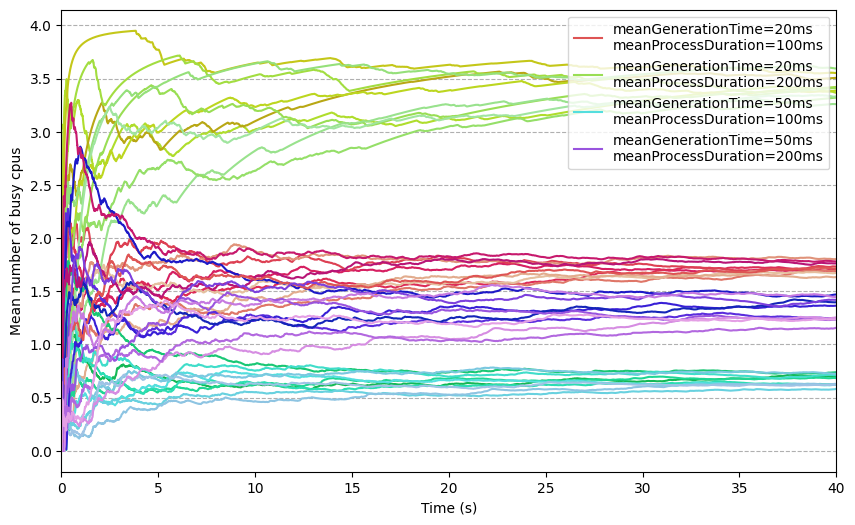
\includegraphics[width=0.9\textwidth]{./images/04/lineWarmup.png}
    \captionof{figure}{Line chart of the mean number of busy CPUs over time for different configurations of meanGenerationTime and meanProcessDuration and multiple repetitions.}
    \label{fig:lineWarmup}
\end{figure}

\begin{figure}[H]
    \captionsetup{type=figure}
    \centering
    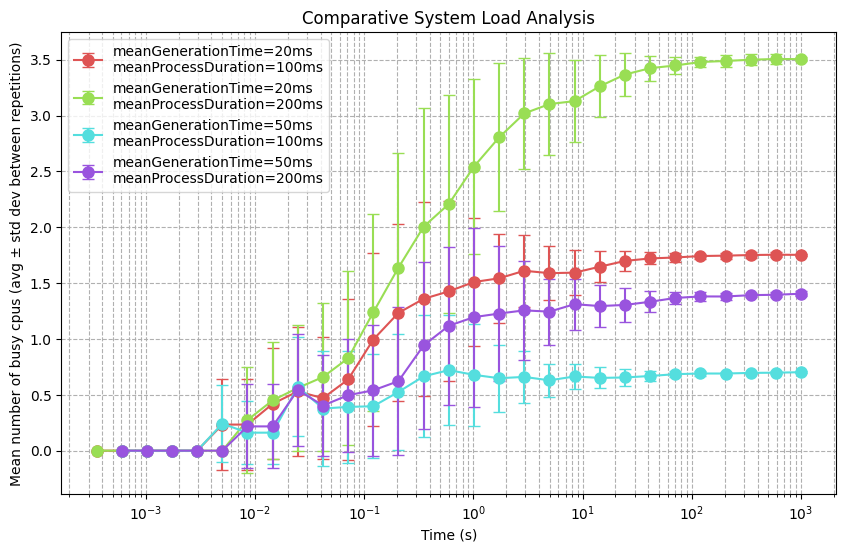
\includegraphics[width=0.9\textwidth]{./images/04/errorWarmup.png}
    \captionof{figure}{Average and Std dev of the mean number of busy CPUs over the repetitions.}
    \label{fig:errorWarmup}
\end{figure}


\begin{table}[H]
    \centering
    \begin{tabular}{c|cc|cc|cc|cc}
                 & \multicolumn{2}{c|}{20ms, 100ms} & \multicolumn{2}{c|}{20ms, 200ms} & \multicolumn{2}{c|}{50ms, 100ms} & \multicolumn{2}{c}{50ms, 200ms}                                   \\
        Time (s) & Avg                              & Std Dev                          & Avg                              & Std Dev                         & Avg  & Std Dev & Avg  & Std Dev \\
        \midrule
        1        & 1.52                             & 0.58                             & 2.54                             & 0.78                            & 0.68 & 0.46    & 1.20 & 0.80    \\
        2        & 1.54                             & 0.37                             & 2.85                             & 0.64                            & 0.67 & 0.27    & 1.25 & 0.51    \\
        5        & 1.59                             & 0.24                             & 3.10                             & 0.46                            & 0.63 & 0.15    & 1.24 & 0.29    \\
        10       & 1.63                             & 0.18                             & 3.18                             & 0.34                            & 0.65 & 0.10    & 1.29 & 0.20    \\
        20       & 1.68                             & 0.11                             & 3.33                             & 0.22                            & 0.64 & 0.08    & 1.27 & 0.15    \\
        50       & 1.72                             & 0.05                             & 3.43                             & 0.10                            & 0.68 & 0.05    & 1.35 & 0.09    \\
        100      & 1.74                             & 0.02                             & 3.47                             & 0.05                            & 0.69 & 0.02    & 1.37 & 0.04    \\
        200      & 1.75                             & 0.02                             & 3.49                             & 0.05                            & 0.69 & 0.02    & 1.38 & 0.03    \\
        500      & 1.75                             & 0.03                             & 3.50                             & 0.05                            & 0.70 & 0.01    & 1.40 & 0.02    \\
        1000     & 1.75                             & 0.01                             & 3.51                             & 0.02                            & 0.70 & 0.01    & 1.41 & 0.02    \\
    \end{tabular}
    \caption{Average and Std dev of the mean number of busy CPUs over the repetitions.}
    \label{tab:stabilization}
\end{table}

\subsection{Simulation duration}

For the simulation duration, we chose to end it at \SI{1000}{\second}. This ensures that after discarding the initial \SI{200}{\second} warm-up period, there remains \SI{800}{\second} of simulation data for analysis. Given that the mean generation time is on the order of tenths of seconds, this duration strikes a balance between obtaining statistically meaningful results even after subsampling and maintaining reasonable simulation times.


\section{Subsampling}

To analyze the data, the assumption of IID-ness will be needed, but without further modification the samples do not uphold it.
For instance, if a process finishes with a large turnaround time, which is caused by a long queue, it is likely that the same thing will happen for the next processes.

To address this and ensure independence between samples, subsampling has been employed. The new sample is constructed taking each point of the starting sample with probability $p$.
$p = \frac{1}{2^k}$ and $k$ is the smallest integer that passes the Ljung-Box test.
Using the Ljung-Box test makes it possible to automate the subsampling step. It was implmented to test the first 30 lags, with a significance level of 5\%, with these values the sample is considered independent if:
\vspace{-0.5\baselineskip}
\begin{equation}
    Q = n(n+2) \sum_{k=1}^{30} \frac{\hat{\rho}_k^2}{n-k} < \chi^2_{0.95,30} \approx 43.77
\end{equation}
The closer the system is to saturation, the stronger the correlation becomes as it can be seen in \cref{fig:autoCorComparison}.

% todo dare nomi ai grafici con metrica che ti dice quanto saturo (bello se definita nella parte iniziale)
\begin{figure}[H]
    \captionsetup{type=figure}
    \centering
    \begin{subfigure}[b]{0.45\textwidth}
        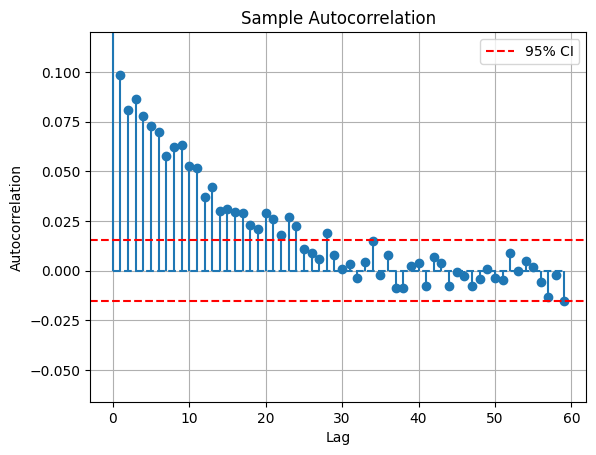
\includegraphics[width=\textwidth]{./images/04/autoCorHighUnfix.png}
        \caption{System close to saturation. Q = 1099}
        \label{fig:autoCorHighUnfix}
    \end{subfigure}
    \hfill % Add space between the subfigures
    \begin{subfigure}[b]{0.45\textwidth}
        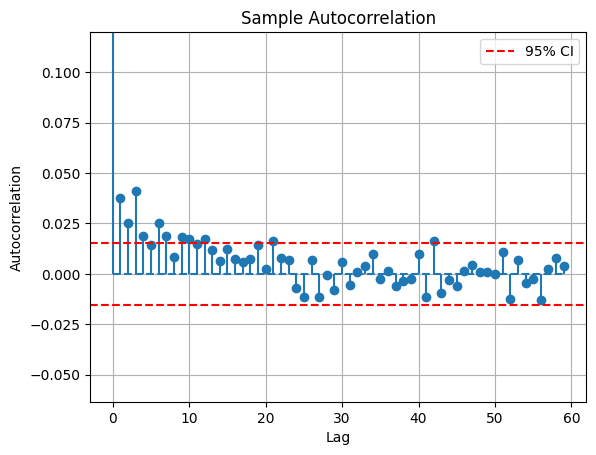
\includegraphics[width=\textwidth]{./images/04/autoCorLowUnfix.png}
        \caption{System with high load. Q = 129}
        \label{fig:autoCorLowUnfix}
    \end{subfigure}
    
    \vspace{10pt} % Add vertical space between the two rows
    
    \begin{subfigure}[b]{0.45\textwidth}
        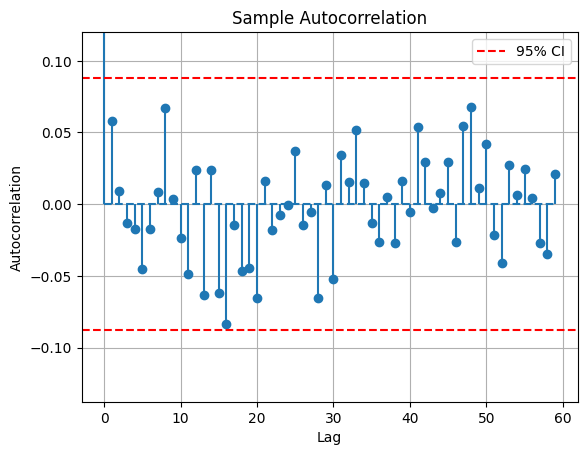
\includegraphics[width=\textwidth]{./images/04/autoCorHighFix.png}
        \caption{System close to saturation with $p=1/16$. Q = 25}
        \label{fig:autoCorHighFix}
    \end{subfigure}
    \hfill % Add space between the subfigures
    \begin{subfigure}[b]{0.45\textwidth}
        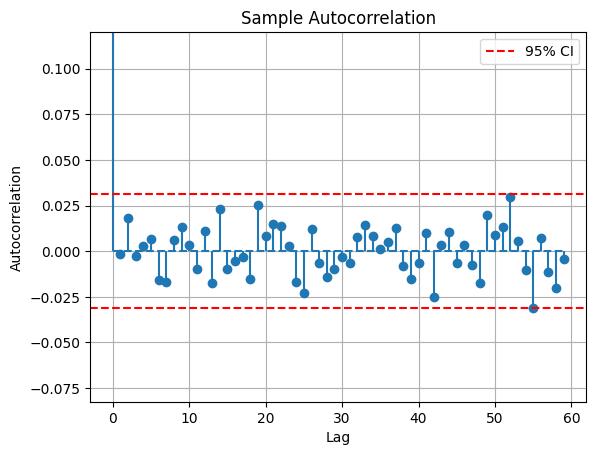
\includegraphics[width=\textwidth]{./images/04/autoCorLowFix.png}
        \caption{System with high load with $p=1/4$. Q = 20}
        \label{fig:autoCorLowFix}
    \end{subfigure}
    
    \vspace{10pt} % Add vertical space before the caption
    \caption{Comparison of turnaround time autocorrelation with and without subsampling for different loads.}
    \label{fig:autoCorComparison}
\end{figure}

\section{Statistical analysis}

For each of our measurements we made sure that the sample variance was stable for different simulation time, proving that the variance of the measurements is finite, and for each of them we collected more than 500 samples. Since after subsampling our observations are IID we can use the central limit theorem to state that:

% todo cambiare e usare direttamente la formula del CI

\begin{equation}
    Z = \frac{\overline{X} - \mu}{\frac{S}{\sqrt{n}}} \sim N(0,1)
\end{equation}

We chose to use a confidence interval of 95\% for our analysis.

\chapter{Conclusions}

% \section{Introduction Example}

\lipsum[1-3]

\begin{code}
    \mintedCode{cpp}{listings/example/test.cpp}
    \captionof{listing}{\texttt{test.cpp}}
    \label{code:test}
\end{code}

\lipsum[66]

\cuno{Commento 1}

\cdue{Commento 2}

Test cite \supercite{GOOGLE}.

Test footnote\footnote{Footnote}.

\begin{figure}[h]
    \captionsetup{type=figure}
    \centering
    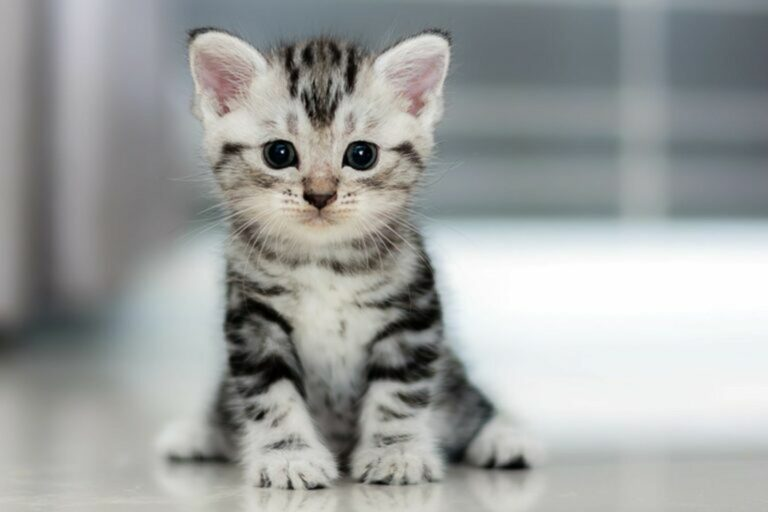
\includegraphics[width=0.9\textwidth]{./images/example/gattino.png}
    \captionof{figure}{Un gattino.}
    \label{fig:gattino}
\end{figure}

Ciao

\lipsum[66]

% Cite sources that are not cited in the text
% \nocite{*}
\printbibliography

\end{document}

%----------------------------------------------------
